\documentclass{beamer}
  % Beamer settings
  \usetheme{Berkeley}
  \usecolortheme{dove}
  \usecolortheme{rose}
  \usefonttheme{professionalfonts}
  \usefonttheme{serif}

  % Packages and settings
  \usepackage{fontspec}
    \setmainfont{Charis SIL}
  \usepackage{hyperref}
    \hypersetup{
      colorlinks=true,
      allcolors=blue
    }
  \usepackage{graphicx}
    \graphicspath{{figures/}}
  \usepackage[style=apa, backend=biber]{biblatex}
    \addbibresource{References.bib}

  % Custom commands
  \newcommand{\orth}[1]{
    $\langle$#1$\rangle$
  }

  % Document information
  \author{Joshua McNeill}
  \title{Summary of Eisenstein and R̆ehůr̆ek \& Kolkus (2009)}
  \date{7 October 2020}

\begin{document}
  \begin{frame}
    \titlepage
  \end{frame}

  \begin{frame}
    \tableofcontents[hideallsubsections]
  \end{frame}

  \AtBeginSection[]{
    \begin{frame}
      \tableofcontents[
        currentsection,
        hideallsubsections
      ]
    \end{frame}
  }

  \section{Language Models}
    \newcommand{\subone}{What are they?}
    \subsection{\subone}
      \begin{frame}{\subone}
        \begin{block}{The probability of a document given some tokens}
          \begin{itemize}
            \item $p(w_1, w_2, \ldots, w_m)$
            \item $w_m \in V$
            \item $V = \{ \text{aardvark}, \text{abacus}, \ldots, \text{zither} \}$
          \end{itemize}
        \end{block}
      \end{frame}

      \begin{frame}{\subone}
        \begin{block}{What good is this?}
          Lets us generate strings
          {\small
            \begin{itemize}
              \item $p ( \text{coffee} | \text{I love dark} )$
            \end{itemize}
          }
          Lets us compare strings
          {\small
            \begin{itemize}
              \item $p ( \text{the coffee black me pleases much} ) < p ( \text{I love dark coffee} )$
            \end{itemize}
          }
        \end{block}
      \end{frame}

    \newcommand{\subtwo}{$n$-gram models}
    \subsection{\subtwo}
      \begin{frame}{\subtwo}
        \begin{block}{A relative frequency approach}
          $p ( \text{Computers are useless, they only give you answers} )$
          \begin{itemize}
            \item[=] $\frac{count(\text{Computers are useless, they only give you answers})}
                        {count(\text{all sentences ever spoken})} $
          \end{itemize}
        \end{block}
        \begin{alertblock}{}
          Impossible to give the latter count
        \end{alertblock}
      \end{frame}

      \begin{frame}{\subtwo}
        \begin{block}{The chain rule}
          {\small
            \begin{itemize}
              \item[] $p ( \text{string} )$
              \item[] $= p ( w_1, w_2, \ldots, w_m )$
              \item[] $= p ( w_1 ) \times p ( w_2 | w_1 ) \times p ( w_3 | w_2, w_1 ) \times \ldots \times p ( w_m | w_{m-1}, \ldots, w_1 )$
            \end{itemize}
          }
        \end{block}

        \begin{block}{Simplified into an $n$-gram model}
          {\small
            \begin{itemize}
              \item[] $\prod_m^M{ p ( w_m | w_{m-1}, \ldots, w_{m-n+1} ) }$
            \end{itemize}
          }
        \end{block}
      \end{frame}

      \begin{frame}{\subtwo}
        \begin{block}{Bigram for ``I like black coffee''}
          {\small
            \begin{itemize}
              \item[] $p ( \text{I} | \# ) \times p ( \text{like} | \text{I} ) \times p ( \text{black} | \text{like} ) \times p ( \text{coffee} | \text{black} )$
            \end{itemize}
          }
        \end{block}

        \begin{block}{}
          Each bigram's individual probability is estimated from the relative frequency in some text
        \end{block}
      \end{frame}

      \begin{frame}{\subtwo}
        \begin{block}{$n$-gram sizes}
          Too small:
          \begin{itemize}
            \item Long distance dependencies are lost
            \item ``\alert{Gorillas} always like to groom \alert{their} friends''
          \end{itemize}
          Too big:
          \begin{itemize}
            \item Data is too sparse to get meaningful counts
            \item How many times does the gorilla 7-gram show up?
          \end{itemize}
        \end{block}
      \end{frame}

    \newcommand{\subthree}{Dealing with sparse data}
    \subsection{\subthree}
      \begin{frame}{\subthree}
        \begin{block}{Smoothing, one solution}
          Laplace smoothing: Add an imaginary count of 1 to all counts
          \begin{itemize}
            \item e.g., bigrams
            \item[] $p_{\text{smooth}} ( w_m | w_{m-1} )$
            \item[=] $\frac{count ( w_{m-1}, w_m ) + 1}
                           {\sum_{w' \in V}{count ( w_{m-1}, w' ) + 1}}$
          \end{itemize}
        \end{block}

        \begin{block}{}
          This is known as additive smoothing and different values can be used
          \begin{itemize}
            \item Jeffreys-Perks law: 0.5
          \end{itemize}
        \end{block}
      \end{frame}

      \begin{frame}{\subthree}
        \begin{block}{Discounting, another solution}
          Take some ``probability mass'' from observed $n$-grams and redistribute it to unobserved $n$-grams
        \end{block}
        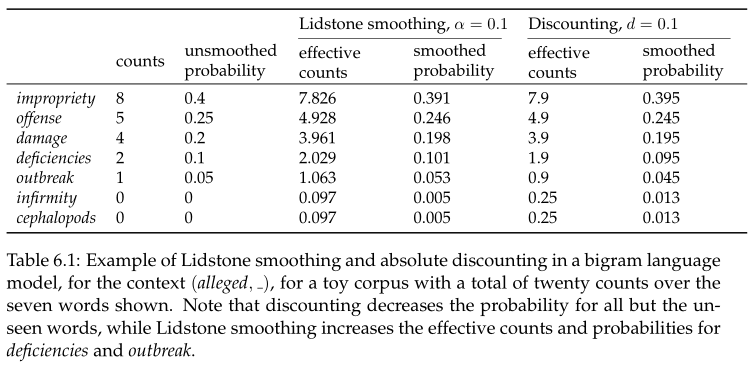
\includegraphics[scale=0.5]{smooth_discount.png}
      \end{frame}

      \begin{frame}{\subthree}
        \begin{block}{Backoff, yet another solution}
          Katz backoff: When a count is 0, use a count from a smaller $n$-gram
          \begin{itemize}
            \item e.g., No counts for the ``like black coffee'' trigram, use the count for the ``black coffee'' bigram instead
          \end{itemize}
        \end{block}
      \end{frame}

      \begin{frame}{\subthree}
        \begin{block}{Interpolation, and another}
          Take a weighted average of counts from all $n$-gram sizes
          \begin{itemize}
            \item[] $p_{\text{interpolation}} ( w_m | w_{m-1}, w_{m-2} )$
            \item[=] $\lambda_3 p_3^* ( w_m | w_{m-1}, w_{m-2} )$
            \item[+] $\lambda_2 p_2^* ( w_m | w_{m-1} )$
            \item[+] $\lambda_1 p_1^* ( w_m )$
          \end{itemize}
          $\lambda$ is the weight
        \end{block}
      \end{frame}

      \begin{frame}{\subthree}
        \begin{block}{Kneser-Ney smoothing, the ``state of the art''}
          Backoff with the incorporation of versatility via a continuation probability
          \begin{itemize}
            \item How many longer $n$-grams does this shorter $n$-gram complete?
          \end{itemize}
        \end{block}
        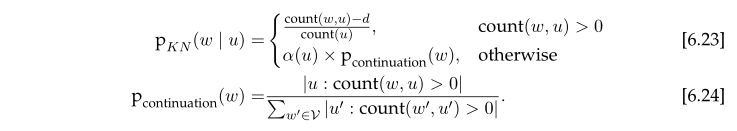
\includegraphics[scale=0.5]{kneser-ney.png}
      \end{frame}

  \section{Language Identification}
    \newcommand{\subfive}{R̆ehůr̆ek \& Kolkus's objective}
    \subsection{\subfive}
      \begin{frame}{\subfive}
        \begin{block}{}
          Improve on language identification of web pages by addressing the following shortcomings of current solutions:
          \begin{itemize}
            \item Dealing with short texts
            \item Dealing with unknown languages
            \item Dealing with multiple languages in one text
            \item Dealing with closely related languages
          \end{itemize}
        \end{block}
      \end{frame}

    \newcommand{\subsix}{Related work}
    \subsection{\subsix}
      \begin{frame}{\subsix}
        \begin{block}{The common words approach}
          \begin{enumerate}
            \item Classify texts by language by hand
            \item Count up function words in those texts
            \item Compare counts to new texts to estimate a match
          \end{enumerate}
        \end{block}
      \end{frame}

      \begin{frame}{\subsix}
        \begin{block}{The character-based $n$-gram language model approach}
          e.g., For \orth{coffee}, \orth{c} is a unigram, \orth{co} a bigram, \orth{cof} a trigram, etc.
          \begin{enumerate}
            \item Classify texts by language by hand
            \item Get counts for character $n$-grams in those texts
            \item Compare counts to new texts to estimate a match
          \end{enumerate}
        \end{block}
        \begin{block}{\textcite{dunning_statistical_1994}}
          Suggests trigram models are optimal
          \begin{itemize}
            \item \textcite{grefenstette_comparing_1995} showed similar performance with common words models
          \end{itemize}
        \end{block}
      \end{frame}

      \begin{frame}{\subsix}
        \begin{block}{Advantages of the character $n$-gram approach}
          \begin{itemize}
            \item Fast convergence (little training data is needed)
            \item Robust (no issues with neologisms, spelling errors, etc.)
            \item Domain independent (no need to tokenize, useful for Asian languages)
          \end{itemize}
        \end{block}
      \end{frame}

      \begin{frame}{\subsix}
        \begin{block}{Factors influencing performance}
          \begin{itemize}
            \item Size of training data
            \begin{itemize}
              \item Too small is bad but so is too large (e.g., overfitting)
            \end{itemize}
            \item Size of input text needed to predict language
            \begin{itemize}
              \item Small amount $\to$ Up to 30 characters/5 words
              \item Large amount $\to$ Over 300 characters/50 words
            \end{itemize}
          \end{itemize}
        \end{block}
      \end{frame}

    \newcommand{\subseven}{Proposed method}
    \subsection{\subseven}
      \begin{frame}{\subseven}
        \begin{block}{The issues, again}
          \begin{enumerate}
            \item Dealing with short texts
            \item Dealing with unknown languages
            \item Dealing with multiple languages in one text
            \item Dealing with closely related languages
          \end{enumerate}
        \end{block}
        \begin{block}{More specifically...}
          \begin{itemize}
            \item For (2), a ``theoretically unfounded'' solution is to train an unknown language from random texts, but doesn't work well
            \item Web pages contain extraneous repeated strings such as \orth{In reply to:}
          \end{itemize}
        \end{block}
      \end{frame}

      \begin{frame}{\subseven}
        \begin{block}{Return to a dictionary method (e.g., common words)}
          $n$-gram advantages not relevant for the current application
          \begin{itemize}
            \item Fast convergence: Corpora availability and retrieval techniques make data highly available
            \item Domain independence: Languages are all Latin character-based
          \end{itemize}
        \end{block}
      \end{frame}

      \begin{frame}{\subseven}
        \begin{block}{Relevance, not commonness}
          Words are measured for how indicative they are of a language
          \begin{itemize}
            \item Positive values: Indicative of language
            \item Near-zero values: No correlation
            \item Negative values: Absence of language
          \end{itemize}
        \end{block}
      \end{frame}

      \begin{frame}{\subseven}
        \begin{block}{Components}
          \begin{itemize}
            \item $C_{\text{lang}}$: Corpus of documents in a language
            \item $C_{\text{lang}_0}$: Background corpus
            \begin{itemize}
              \item Union of all documents in all languages
            \end{itemize}
          \end{itemize}
        \end{block}
        \begin{block}{Uncorrected observed frequencies for word $w$}
          {\small
            \begin{itemize}
              \item $\bar{g}_{lang}(w) = \frac{TF(w, C_{\text{lang}})}
                                              {\#(C_{\text{lang}})}$
              \item $g_{0}(w) = \frac{TF(w, C_{0})}
                                     {\#(C_{0})}$
            \end{itemize}
          }
          Correction is done using Jelinek-Mercer smoothing
        \end{block}
      \end{frame}

      \begin{frame}{\subseven}
        \begin{block}{Final formula}
          \begin{itemize}
            \item[] $\sum_{g_{L}(w_i)<<g_{\text{lang}}(w_i)}f_i \cdot \text{rel}(w_i, \text{lang})$
          \end{itemize}
          Where...
          \begin{itemize}
            \item[] $\text{rel}(w_i, \text{lang}) = log(g_{\text{lang}}(w)) - log(g_{0}(w))$
            \item[] $f_i$ is an instance of word $w$
          \end{itemize}
          Normalized by dividing by the frequency of words in the document
        \end{block}
      \end{frame}

      \begin{frame}{\subseven}
        \begin{block}{Identifying the language}
          \begin{itemize}
            \item Set a threshold score $t$ for each language
            \item $F_1$ applied to held out data is one candidate for $t$
          \end{itemize}
        \end{block}
      \end{frame}

    \newcommand{\subeight}{Practical considerations}
    \subsection{\subeight}
      \begin{frame}{\subeight}
        \begin{block}{}
          \begin{itemize}
            \item Algorithm speed: ``[E]xtremely fast''
            \item Memory: About equivalent to a pentagram model
            \begin{itemize}
              \item Only language distinctive words need be stored
            \end{itemize}
            \item Corpora sizes: Wikipedia dumps, so GBs each
          \end{itemize}
        \end{block}
      \end{frame}

    \newcommand{\subnine}{Evaluation}
    \subsection{\subnine}
      \begin{frame}{\subnine}
        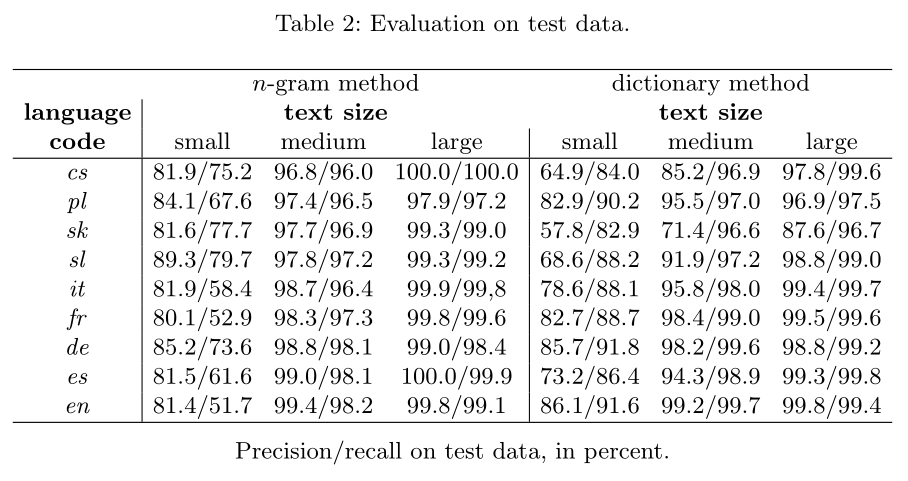
\includegraphics[scale=0.4]{evaluation.png}
      \end{frame}

    \newcommand{\subten}{Addendum: Segmenting for language}
    \subsection{\subten}
      \begin{frame}{\subten}
        \begin{block}{Process}
          \begin{enumerate}
            \item They use word relevancies to create a signal
            \item This signal is smoothed using the median in a window of size 2
            \item Local minima are used as possible language segment boundaries
          \end{enumerate}
        \end{block}
        \begin{block}{Evaluation}
          97.16\% accuracy (1,420 misclassified words out of 49,943)
          \begin{itemize}
            \item 603 boundaries were off by one word only
          \end{itemize}
        \end{block}
      \end{frame}
\end{document}
